% ------- textdoclet_include/finish.tex



\section{verwendetes Datenbankschema}
Das System persistiert Daten in einer zentralen MySQL-Datenbank auf dem Tomcat-Server und zusätzlich auf einer lokalen SQLite-Datenbank auf den Clients. Beide Datenbanken verwenden das gleiche Schema.\\

\section{Client-Server-Schnittstelle}
Dieser Abschnitt erläutert die Schnittstelle zwischen dem Client und dem Server. Diese Schnittstelle besteht aus zwei Teilen:

Zum Einen bietet der Server eine REST API an, über die der Client die Dienste des Servers in Anspruch nehmen kann. Zum Anderen gibt es eine Schnittstelle, die über Firebase Cloud Messaging realisiert ist, damit der Server Nachrichten an bestimmte Clients schicken kann.

\subsection{REST API des Servers}
Folgende Grafik zeigt, welche Methoden unter welchen URL des Servers zu erreichen sind:
\begin{figure}[H]
	\centering
	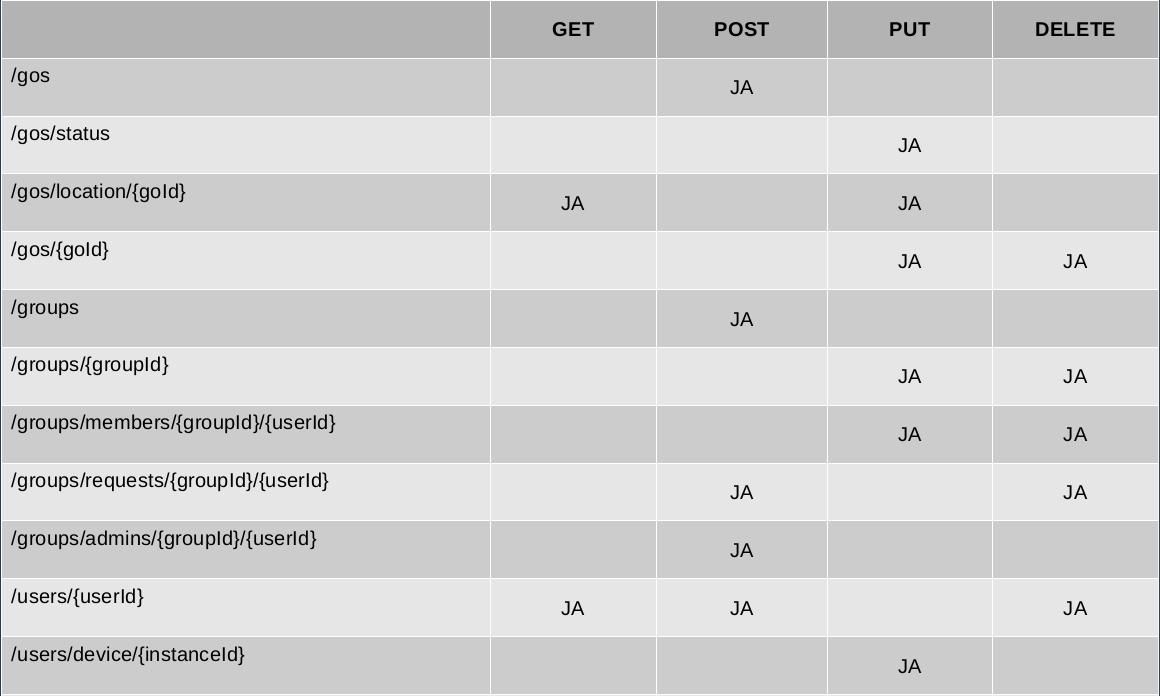
\includegraphics[width=0.8\textwidth]{restapi.png}
	\caption{Übersicht über die Rest Api des Servers}
\end{figure}
Aufrufe der Request-Methoden DELETE und GET enthalten keinen Content-Body. Sämtliche Informationen, die der Server braucht, um richtig auf die anfrage antworten zu können, sind in der URL kodiert.
Bei den Methoden POST und PUT, sowie bei Antworten des Servers, die einen Content-Body erfordern, ist sind die Daten in einem JSON-Objekt gekapselt. Dieses Objekt wird von dem Framework Gson aus der entsprechenden Entity-Klasse erzeugt. die Anwendung muss den genauen Aufbau des JSON Objekts nicht kennen. Die Verantwortung für die Verwaltung derselben wird hier vollständig an Gson übergeben.

Bei sämtlichen Requests kann der Client anhand des HTTP-Statuscodes der Server-Response erkennen, ob die Anfrage erfolgreich ausgeführt werden konnte.

\subsection{FCM Schnittstelle}
Die Schnittstelle zwischen Server und Client, die zum Senden von Downstream-Nachrichten verwenet werden kann, wird über Firease Cloud Messaging realisiert. Der Server sendet einen HTTP Post Request an den Firebase Server. Dabei besteht der Content-Body dieser HTTP-Anfrage aus einem JSON-Objekt indem der Empfänger und die zu übermittlenden Daten spezifiziert sind.

Folgende Grafik \footnote{Quelle: https://firebase.google.com/docs/cloud-messaging/send-message} zeigt den Aufbau eines HTTP-Requests, wie er an den FCM Server gesendet werden muss für eine erfolgreiche Weiterleitung der Nachricht:

\begin{figure}[H]
	\centering
	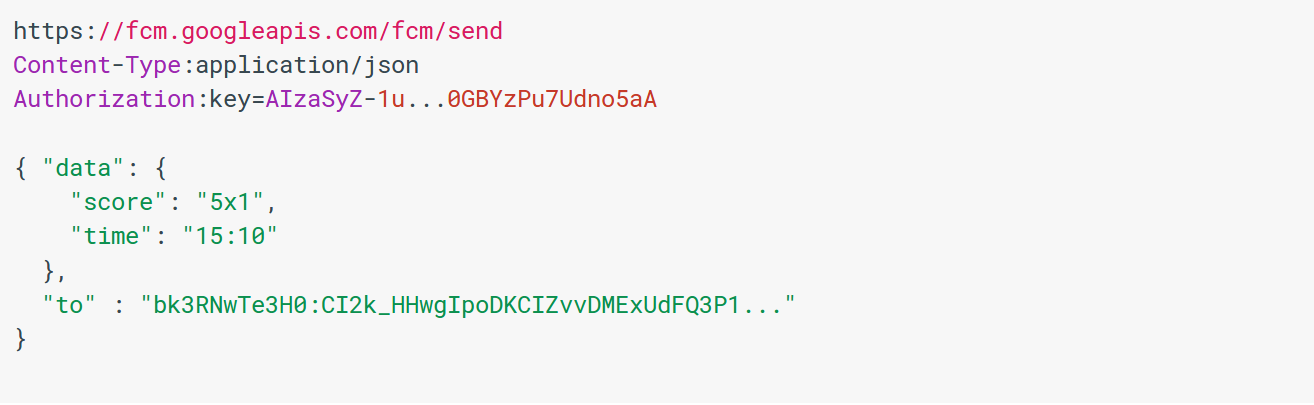
\includegraphics[width=1\textwidth]{http_format.png}
	\caption{Beispiel für ein HTTP-Request an den FCM Server}
\end{figure}

Das in grün markierte JSON-Objekt kann dabei je nach Anwendungsfall ein anderes Data-Field enthalten. Das "to"-Feld enthält die instanceId des Empfängers der Nachricht.

\textbf{Inhalt des 'data'-Felds für die verschiedenen Anwendungsfälle der App:}
Zunächst enthalten sämtliche Nachrichten unter dem Tag "tag" einen String der signalisiert, was der Anlass zum Senden der Nachricht war. Bei diesen Strings handelt es sich um Elemente des Enums EventArg.
\begin{itemize}
	\item \textit{Go Added}\\
	Ein aus einer GO-Entität erzeugtes JSON-Objekt unter dem Tag 'go'. Dieses wird automatisch durch das Framework Gson erzeugt.
	\item \textit{Go Edited}\\
	Ein aus einer GO-Entität erzeugtes JSON-Objekt unter dem Tag 'go'. Dieses wird automatisch durch das Framework Gson erzeugt. Es werden allerdings die Listen der Go-Teilnehmer aus dem Objekt entfernt,
	da Änderungen derselben von diesem Anwendungsfall nicht betroffen sind und die Daten somit nicht übertragen werden müssen.
	\item \textit{Go Removed}\\
	Die ID des entfernten Gos unter dem Tag 'id'
	\item \textit{Group Edited}\\
	Ein aus einer Group-Entität erzeugtes JSON-Objekt unter dem Tag 'group'. Dieses wird automatisch durch das Framework Gson erzeugt. Es werden allerdings die Listen der Gruppenmitgleider und Administratoren aus dem Objekt entfernt, da Änderungen derselben von diesem Anwendungsfall nicht betroffen sind und die Daten somit nicht übertragen werden müssen.
	\item \textit{Group Removed}\\
	Die ID der entfernten Gruppe unter dem Tag 'id'
	\item \textit{Group Request Received}\\
	Ein aus einer Group-Entität erzeugtes JSON-Objekt unter dem Tag 'group'. Dieses wird automatisch durch das Framework Gson erzeugt
	\item \textit{Member Added}\\
	Die ID der Gruppe zu der der Benutzer hinzugefügt werden soll unter dem Tag 'id'. Unter dem Tag 'user' ist ein JSON-Objekt gespeichert, das aus einer User-Entität erzeigt wurde. Dies geschieht automatisch durch das Framework Gson.
	\item \textit{Member Removed}\\
	Die ID des Benutzers, der aus der Gruppe entfernt werden soll unter dem Tag 'user\_id' und die ID der Gruppe, aus der der Benutzer entfernt werden soll unter dem Tag 'group\_id'.
	\item \textit{Admin Added}\\
	Die ID des Benutzers, der als Adminsitrator hinzugefügt werden soll unter dem Tag 'user\_id' und die ID der Gruppe, in der dies geschehen soll unter dem Tag 'group\_id'. Es ist nicht nötig das vollständige User-Objekt zu senden, da dies bereits auf den Clients in dem entsprechenden Gruppen-Objekt gespeichert ist.
	\item \textit{Status Changed}\\
	Die ID des Benutzers, der seinen Status geändert hat unter dem Tag 'user\_id', die ID des GOs in der die Statusänderung stattgefunden hat unter dem Tag 'go\_id' und eine Zahl, die den neuen Status repräsentiert, unter dem Tag 'status'. Es gilt '0': ABELEHNT, '1': BESTÄTIGT, '2': UNTERWEGS.
\end{itemize}

Bei den Clients kommt die gesendete Nachricht als remoteMessage-Objekt an. Durch die getData()-Methode kann auf den Content-Body, also das JSON-Objekt, das den eigentlichen Inhalte der Nachricht entält zugegriffen werden.



\section{Klassendiagramme}

\section{Sequenzdiagramme}

\subsection{Hinzufügen eines Gruppenmitglieds}

\begin{figure}[H]
	\centering
	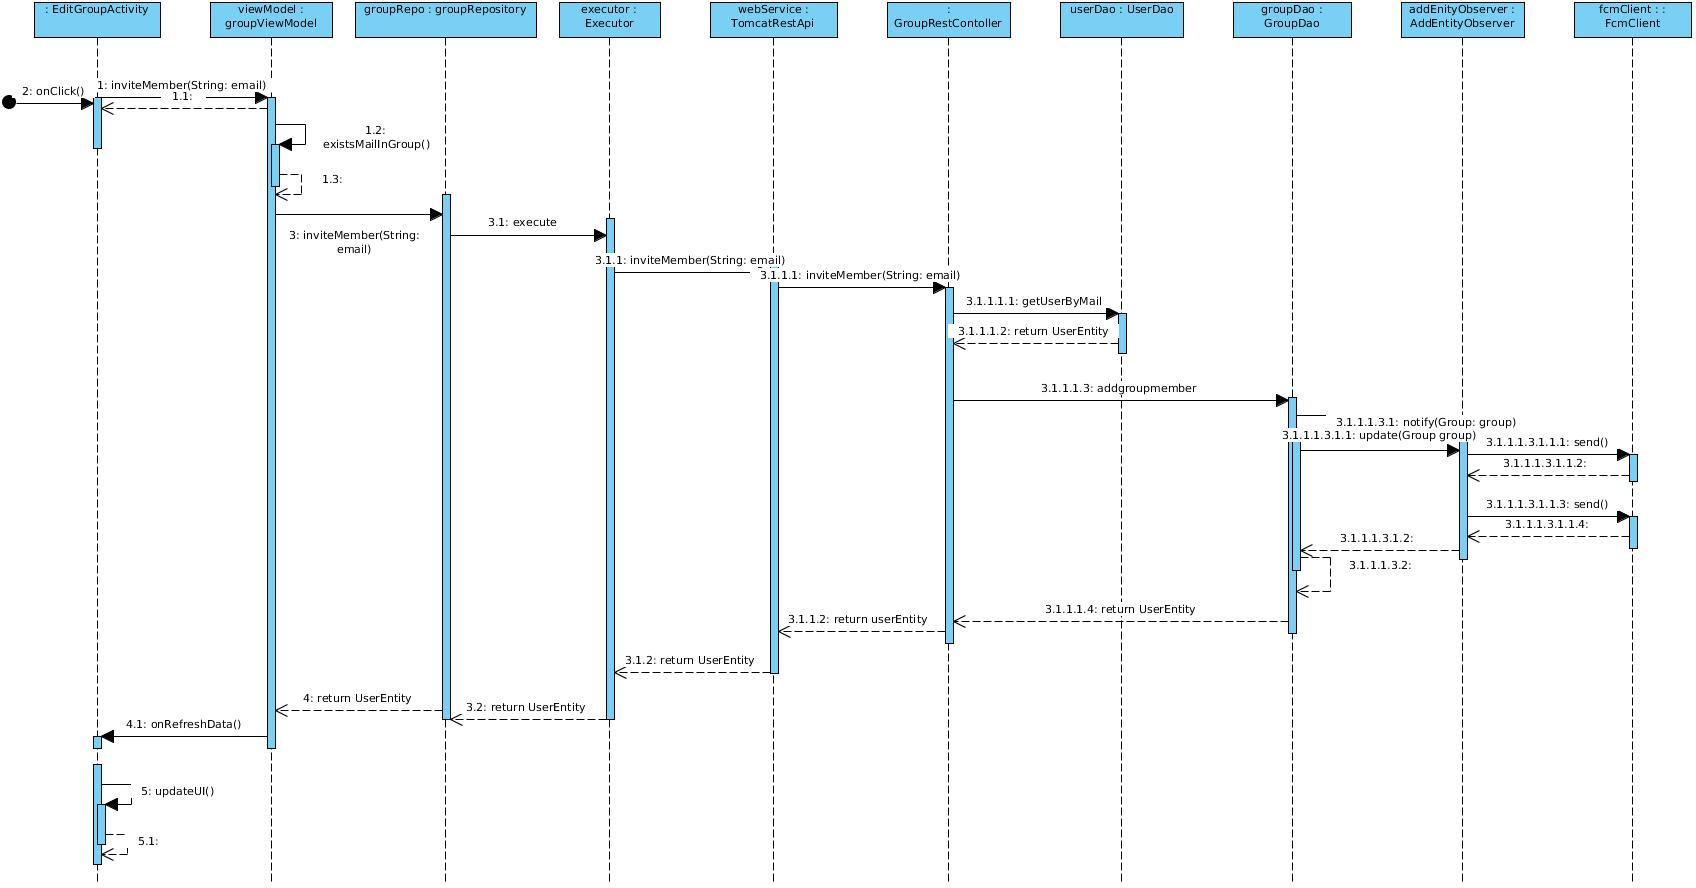
\includegraphics[width=1\textwidth]{../Sequenzdiagramme/addGroupMember.jpg}
	\caption{Sequenzdiagramm - Hinzufügen eines Gruppenmitglieds Teil 1}
\end{figure}

Das obige Sequenzdiagramm zeigt, was während der Ausführung des Programms passiert, wenn ein Benutzer die Funktion "inviteMember" ausführt. Das User Interface stellt dem Benutzer ein Textfeld zur Eingabe der E-Mailadresse und einen Button zum Bestätigen zur Verfügung. Bei Klick dieses Buttons extrahiert die Activity-Klasse die eingegebene Mail-Adresse aus dem Textfeld und übergibt diese an das ViewModel über den Methodenaufruf "inviteMember". Das ViewModel überprüft zunächst ob es bereits einen Benutzer in Gruppe gibt, der diese E-Mailadresse besitzt. Falls nicht, wird die Gruppeneinladung an die Grouprepository weitergeleitet und von dort über die Klasse TomcatrestApi an den Server gesendet.

Empfängt der Server eine Anfrage, einen User zu einer Gruppe hinzuzufügen, wird diese Anfrage zunächst an das UserDao weitergegeben. Dort wird zuerst die Methode getUserByMail() aufgerufen, um den richtigen Benutzer aus der Datenbank zu finden. Danach wird die addGroupmember-methode des GroupDaos aufgerufen. In dieser methode wird die neue gruppenanfrage in der Datenbank gespeichert und es werden die Observer benachrichtigt, dass sich Daten geändert haben.

Der AddEntityObserver erkennt, dass es sich um eine Änderung handelt, die seinen Veratnwortlichkeitsbereich betrifft. Er bekommt beim Aufruf der update()-Methode die Gruppe mit der zusätzlichen Gruppenanfrage übergeben. Der Observer extrahiert alle Gruppenmitglieder aus dem Gruppenobjekt und ruft die send()-methode des FcmClients auf, um das geänderte Gruppenobjekt an alle Gruppenmitglieder zu senden. Danach wird die send()-Methode ein zweites Mal aufgerufen, um dem neuen Gruppenmitglied die neue Gruppenanfrage zu übermitteln.

\begin{figure}[H]
	\centering
	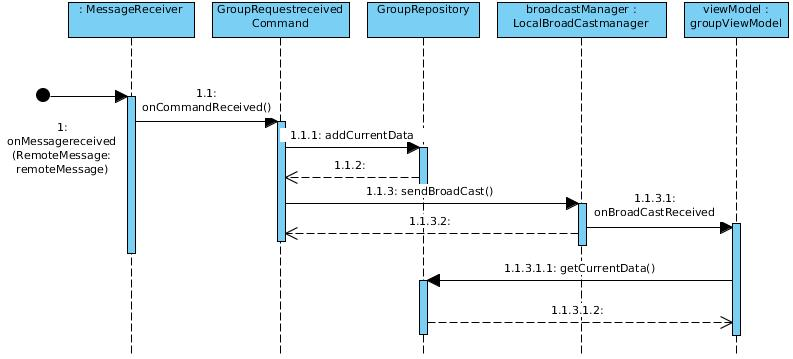
\includegraphics[width=1\textwidth]{../Sequenzdiagramme/addMember2.jpg}
	\caption{Sequenzdiagramm - Hinzufügen eines Gruppenmitglieds Teil 2}
\end{figure}

Das zweite Sequenzdiagramm zeigt, was passiert, wenn an einen Benutzer eine Gruppenmitgliedschaftsanfrage gesendet wird. Die Nachricht, die von dem Server, über dem Firebase Cloud Messaging Server, an den Client gesendet wird, löst einen Aufruf der Methode onMessageReceived() in der Klasse MessageReceiver aus. Diese Klasse extrahiert das JSON-Feld COMMAND\_CODE aus dem empfangenen JSON-Objekt und findet so heraus, an welches ServerCommand-Objekt die Anfrage weitergeleitet werden muss.

Nach Weiterleitung der Anfrage an den GroupRequestReceivedCommand wird dort das Datenfeld aus der JSON-Nachricht extrahiert. dort ist die Gruppe gespeichert, zu der er Benutzer eingeladen wurde. Diese Gruppe wird in dem öffentlichen "CurrentData" Field des GroupRepository gespeichert. Danach schickt das GroupRequestReceivedCommand-Objekt einen Broadcast an alle ViewModels. Das GroupViewModel erkennt, dass der Broadcast eine Änderung der Gruppen des Benutzers betrifft. Daher wird dort die onBroadcastReceived()-Methode auferufen. Daraufhin holt sich das ViewModel die aktualisierten Daten von der GoupRepository ab, durch einen Aufruf der getCurrentData()-Methode. Da das UI die LiveData der ViewModels beobachtet, wird automatisch bei einer Aktualisierung des ViewModels auch das UI aktualisiert und zeigt die neuen Daten an.

\subsection{Entfernen einer Gruppe}

\begin{figure}[H]
	\centering
	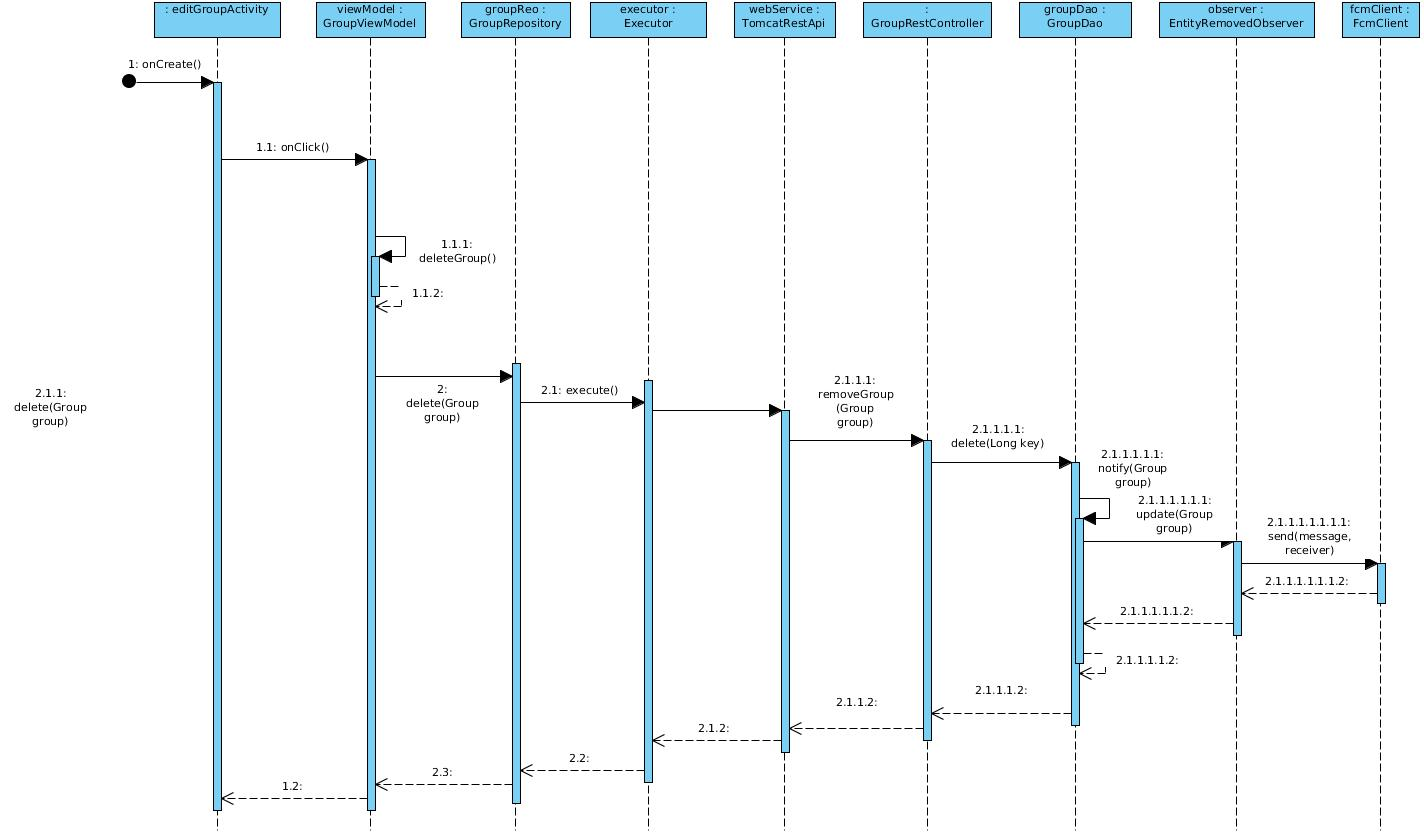
\includegraphics[width=1\textwidth]{../Sequenzdiagramme/deleteGroup_sequenz.jpg}
	\caption{Sequenzdiagramm - Entfernen einer Gruppe}
\end{figure}

Das obige Sequenzdiagramm zeigt den Programmablauf, nachdem ein Benutzer die "Gruppe löschen"-Funktion ausgelöst hat. Das UI gibt den Button Press an das GroupViewModel weiter. Dort wird die Gruppe zunächst in den lokaeln Daten gelöscht. Dabei muss sichergestellt werden, dass die Daten nach dem Löschen konsistent sind, also z.B. auch alle GOs der Gruppe gelöscht wurden.

Danahc wird die Anfrage über die GroupRepository und das Rest API an den Server übergeben, wo sie durch den Methodenaufruf deleteGroup() in der GroupRestController-Klasse ankommt. Von dort aus wird die Anfrage an das GroupDao gegeben, welches die Gruppe in der Datenbank löscht. Auch hier muss auf die Konsistenz der Daten geachtet werden. Danach werden die Observer des GroupDaos benachrichtigt, dass eine Ändeurng stattgefunden hat. Da die Änderung nur den EntityRemovedObserver betrifft, wird bei diesem Objekt die Methode update() aufgerufen. Mit dem Methodenaufruf wird auch die gelöschte Gruppe übergeben.

Der Observer baut ein Message-Objekt aus der erhaltenen Gruppe und extrahiert eine Listse aller Gruppenmitglieder aus dem Gruppenobjekt. Diese Daten werden witergegeben an dem FcmClient über die Methode send(). Dadurch werden die Nachrichten über die Löschung der Gruppe an die Gruppenmitglieder geschickt, damit diese ihre lokalen Daten anpassen können.

\section{Finish}{

}
% ------- textdoclet_include/finish.tex end
